\documentclass[11pt, a4paper]{article}

% ==========================================
% PREAMBOLO E CONFIGURAZIONE PACCHETTI
% ==========================================
\usepackage[utf8]{inputenc}
\usepackage[T1]{fontenc}
\usepackage[italian]{babel}
\usepackage{geometry}
\geometry{top=2.5cm, bottom=2.5cm, left=2.5cm, right=2.5cm}
\usepackage{hyperref}
\usepackage{enumitem}
\usepackage{xcolor}
\usepackage{graphicx}
\usepackage{booktabs}
\usepackage{amsmath}
\usepackage{amssymb}
\usepackage{listings}
\usepackage{caption}
\usepackage{tcolorbox}

% Configurazione dei link ipertestuali
\hypersetup{
    colorlinks=true,
    linkcolor=blue!70!black,
    filecolor=magenta,
    urlcolor=cyan!70!black,
    pdftitle={Relazione Tecnica Approfondita: progettoASM},
    pdfpagemode=FullScreen,
}

% Configurazione per i blocchi di codice
\definecolor{codegray}{rgb}{0.95,0.95,0.95}
\definecolor{codeblue}{rgb}{0.1,0.2,0.8}
\definecolor{codegreen}{rgb}{0.1,0.6,0.2}

\lstset{
    backgroundcolor=\color{codegray},
    commentstyle=\color{codegreen},
    keywordstyle=\color{codeblue}\bfseries,
    numberstyle=\tiny\color{gray},
    stringstyle=\color{magenta},
    basicstyle=\ttfamily\footnotesize,
    breakatwhitespace=false,
    breaklines=true,
    captionpos=b,
    keepspaces=true,
    numbers=left,
    numbersep=5pt,
    showspaces=false,
    showstringspaces=false,
    showtabs=false,
    tabsize=2,
    frame=single,
    rulecolor=\color{gray!40}
}

\title{\textbf{Relazione Tecnica Approfondita: Architettura e Fasi di Esecuzione}\\ \large \texttt{progettoASM} - Studio di Sistemi Agentici in Reti Sociali}
\author{Senior Software Engineer \& Technical Writer}
\date{\today}

\begin{document}

\maketitle

\tableofcontents
\newpage

% ==========================================
% SEZIONE 1: PANORAMICA
% ==========================================
\section{Panoramica del Progetto}

Il repository \href{https://github.com/stefaano19/progettoASM}{\texttt{progettoASM}} implementa un framework sperimentale avanzato per lo studio di un sistema agentico all'interno di reti sociali complesse. Concepito come progetto accademico per il corso di Analisi di Social Network e Media, il sistema si discosta dai tradizionali simulatori statici adottando un approccio di \textbf{co-evoluzione dinamica}.

Il problema centrale esplorato dal progetto è la modellazione realistica di come gli stati interni degli agenti (opinioni testuali e cognitive), la topologia della rete (legami sociali) e gli interventi esterni (come il fact-checking) si influenzino reciprocamente e simultaneamente. Invece di eseguire questi step come pipeline sequenziali e indipendenti, il framework li integra in un ciclo chiuso di interazione continua.

Il target di riferimento include ricercatori nell'ambito della \textit{Network Science}, studiosi di sistemi multi-agente e data scientist. L'uso del dataset \texttt{ogbl-collab} (Open Graph Benchmark), originariamente una rete di co-autoraggio accademico, viene qui sfruttato in modo innovativo per rappresentare un ambiente sociale in cui la prossimità nello spazio vettoriale cognitivo degli agenti determina la probabilità di formazione o recisione dei legami.

% ==========================================
% SEZIONE 2: STACK TECNOLOGICO
% ==========================================
\section{Stack Tecnologico}

Lo stack tecnologico è fortemente orientato al Machine Learning geometrico e al Natural Language Processing generativo, combinando astrazioni algoritmiche complesse con paradigmi di orchestrazione moderni.

\begin{itemize}[leftmargin=*]
    \item \textbf{Linguaggio e Core:} Python ($\ge$ 3.10), scelto per l'ecosistema predominante in ambito Data Science.
    \item \textbf{Graph Neural Networks (GNN):} Utilizzo del modello \textit{GraphSAGE} (Sample and Aggregate). La scelta di SAGE rispetto a GCN standard permette un apprendimento induttivo, fondamentale per grafi la cui topologia muta a ogni tick temporale, evitando di dover riaddestrare la rete da zero per i nuovi nodi o archi.
    \item \textbf{Agenti Generativi (LLM):} Motore di inferenza basato su \textbf{vLLM} (versione 0.30.0), che serve il modello \texttt{casperhansen/llama-3-8b-instruct-awq} distribuito su due GPU T4 in \textit{tensor parallel}. vLLM massimizza il \textit{throughput} grazie al continuous batching e ottimizza l'uso della VRAM, garantendo un'esecuzione rapida e massiva degli agenti senza incorrere nei \textit{rate-limit} tipici delle API cloud esterne e mantenendo la completa sovranità sui dati. Con questa configurazione uno step di simulazione richiede circa 6 minuti.
    \item \textbf{Influenza e Propagazione:} Implementazione del modello \textit{Linear Threshold} per la dinamica di contagio (diffusione di un'opinione/stato), accoppiato a una selezione greedy dei nodi \textit{seed} per l'intervento di fact-checking. L'obiettivo di selezione è allineato alle stesse soglie che governano le transizioni nella simulazione; in alternativa è disponibile l'algoritmo CELF (\textit{Cost-Effective Lazy Forward}) su modello Independent Cascade.
\end{itemize}

% ==========================================
% SEZIONE 3: LE FASI DELLA PIPELINE
% ==========================================
\section{Esecuzione della Pipeline: Analisi delle Fasi}

L'esecuzione del framework è strutturata in un \textit{notebook} orchestratore (\texttt{kaggle\_full\_run.ipynb}) suddiviso logicamente in quattro fasi distinte, progettate per gestire l'intero ciclo di vita della co-evoluzione del sistema agentico.

\begin{figure}[h]
    \centering
    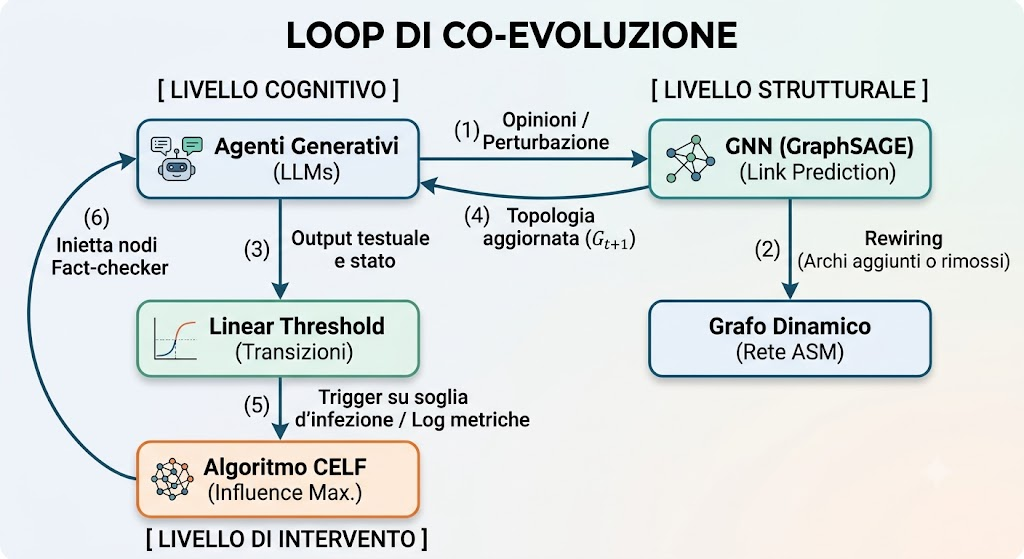
\includegraphics[width=0.85\textwidth]{loop_coevoluzione.png}
    \caption{Schema d'insieme del loop di co-evoluzione. I tre livelli del sistema — cognitivo (Agenti LLM), strutturale (GNN e Grafo Dinamico) e di intervento (Linear Threshold e CELF) — interagiscono in un ciclo chiuso: gli agenti generano opinioni che perturbano gli embedding (1), la GNN calcola il rewiring della topologia (2), il nuovo output testuale alimenta la macchina a stati (3), la topologia aggiornata $G_{t+1}$ retroagisce sugli agenti (4), le transizioni innescano il trigger su soglia d'infezione per CELF (5), che inietta i nodi Fact-Checker richiudendo il ciclo (6).}
    \label{fig:loop-coevoluzione}
\end{figure}

Questo schema fornisce una chiave di lettura trasversale alle quattro fasi descritte di seguito: la Fase 0 prepara il grafo e le baseline su cui il ciclo opererà, la Fase 1 attiva il livello cognitivo (nodo ``Agenti Generativi''), la Fase 2 chiude il ciclo tra livello cognitivo e livello strutturale (archi 1--4), e la Fase 3 introduce il livello di intervento (archi 5--6), completando il loop.

\subsection{Fase 0: Setup Ambiente, Data Ingestion e Baseline}
La Fase 0 si occupa della preparazione dell'infrastruttura computazionale e della profilazione iniziale della rete.
\begin{itemize}[leftmargin=*]
    \item \textbf{Setup Infrastrutturale:} Viene inizializzato in background il server \texttt{vLLM} locale caricando il modello \texttt{casperhansen/llama-3-8b-instruct-awq}. Le versioni delle librerie (\texttt{vllm}, \texttt{transformers}, \texttt{huggingface\_hub}, \texttt{tokenizers}) sono fissate per garantire un ambiente riproducibile. I flag di avvio ottimizzano la memoria della GPU (es. \texttt{--gpu-memory-utilization 0.90}) e distribuiscono il modello su entrambe le GPU (\texttt{--tensor-parallel-size 2}), mentre l'accesso è protetto tramite variabili d'ambiente ricavate dai \textit{Kaggle Secrets}. Se il server non risponde, il notebook interrompe l'esecuzione invece di proseguire senza modello linguistico.
    \item \textbf{Campionamento Topologico:} Il modulo \texttt{data\_loader} importa il dataset completo \texttt{ogbl-collab}. Per renderne trattabile l'elaborazione, l'\texttt{extractor} preleva un sottografo target di 5000 nodi applicando un \textbf{Forest Fire Sampling} (con parametro \texttt{forward\_prob = 0.5}). Questo algoritmo preserva in modo soddisfacente la distribuzione dei gradi, le \textit{community} e il coefficiente di clustering originali.
    \item \textbf{Community Detection e Baseline:} Tramite l'algoritmo di \textit{Label Propagation}, vengono identificate 415 community con un coefficiente di Modularity (Q) estremamente alto (0.8265). Il modulo \texttt{metrics} archivia i KPI di partenza, tra cui l'Echo Chamber Index e le metriche di centralità (Degree, PageRank, Katz).
\end{itemize}

\subsubsection{Approfondimento: i moduli del sottosistema \texttt{graph}}
La Fase 0 si appoggia a quattro moduli fondamentali del sottosistema \texttt{graph}, i quali forniscono rispettivamente le funzionalità di acquisizione del dataset, campionamento del sottografo, community detection e calcolo delle metriche strutturali e di opinione.

\paragraph{data\_loader.py — Data Loader \& Download}
Questo modulo gestisce l'acquisizione del dataset accademico standard \texttt{ogbl-collab} dall'Open Graph Benchmark (OGB) e lo adatta per la simulazione.

\begin{itemize}[leftmargin=*]
    \item \textbf{Caricamento e caching:}
    \begin{itemize}
        \item Cerca prima se esiste il file binario serializzato \texttt{full\_graph.gpickle} in \texttt{data/processed/}. Se lo trova, lo carica all'istante, evitando di riscaricare e ricostruire il grafo e risparmiando minuti di elaborazione.
        \item Se non è presente, scarica il dataset in \texttt{data/raw/} tramite l'API \texttt{LinkPropPredDataset} di OGB.
    \end{itemize}
    \item \textbf{Conversione e costruzione del grafo:}
    \begin{itemize}
        \item Converte la matrice di collegamenti di OGB (\texttt{edge\_index}) in un grafo non orientato NetworkX (\texttt{nx.Graph}).
        \item Associa a ciascun nodo la feature vettoriale Word2Vec a 128 dimensioni, che rappresenta i temi di ricerca degli autori.
    \end{itemize}
    \item \textbf{Filtro temporale:} se \texttt{dataset.year\_filter} è impostato in \texttt{config.yaml}, elimina tutti gli archi creati dopo quell'anno, consentendo di studiare la rete in una specifica finestra storica.
    \item \textbf{Statistiche rapide} (\texttt{graph\_summary}): restituisce informazioni descrittive istantanee sul grafo completo, tra cui numero di nodi/archi, densità, numero di componenti connesse e dimensione della componente connessa principale (LCC).
\end{itemize}

\paragraph{community.py — Community Detection}
Questo modulo si occupa di dividere la rete sociale in gruppi (o partizioni) di nodi densamente connessi tra loro, note come comunità. All'interno del framework, queste comunità costituiscono la struttura topologica di riferimento rispetto alla quale si misura la segregazione strutturale della rete.

\begin{itemize}[leftmargin=*]
    \item \textbf{Algoritmi di partizionamento supportati:}
    \begin{itemize}
        \item \textit{Louvain} (\texttt{\_louvain}): algoritmo euristico che ottimizza in modo iterativo la modularità (Q). Utilizza la funzione nativa di NetworkX ed è lo standard per individuare partizioni stabili.
        \item \textit{Label Propagation} (\texttt{\_label\_propagation}): algoritmo basato sul consenso dei vicini, in cui ogni nodo assume l'etichetta maggioritaria dei suoi adiacenti. È più rapido di Louvain ma meno deterministico.
    \end{itemize}
    \item \textbf{Meccanismo di caching:} per evitare il calcolo superfluo ad ogni avvio della simulazione, la funzione principale \texttt{detect\_communities} verifica l'esistenza del file \texttt{community\_map.json}. Se presente, valida che le dimensioni del grafo corrispondano e carica le comunità dalla cache; altrimenti avvia il calcolo e scrive il file di cache.
    \item \textbf{Analisi statistica} (\texttt{community\_stats}): calcola e restituisce statistiche aggregate sulla qualità e sulla dimensione delle comunità trovate (numero totale di gruppi, dimensione minima, massima, media, deviazione standard e distribuzione dettagliata delle frequenze).
\end{itemize}

\paragraph{extractor.py — Subgraph Extractor}
Il dataset completo \texttt{ogbl-collab} contiene 235\,868 nodi e 967\,632 archi non orientati (2\,358\,104 collaborazioni con timestamp prima della deduplicazione). Simulare una rete agentica LLM su questa scala richiederebbe risorse insostenibili: il modulo \texttt{extractor.py} campiona un sottografo connesso, compatto e strutturalmente rappresentativo per l'esecuzione in locale o in cloud.

\begin{itemize}[leftmargin=*]
    \item \textbf{Algoritmi di campionamento:}
    \begin{itemize}
        \item \textit{Forest Fire} (\texttt{\_forest\_fire\_sample}, default): algoritmo probabilistico ispirato agli incendi boschivi. Preserva bene le proprietà della rete originale (legge di potenza dei gradi, coefficiente di clustering e struttura di comunità).
        \item \textit{BFS} (\texttt{\_bfs\_sample}): esplorazione in ampiezza a partire da un nodo seme, tende a creare ``sfere'' dense.
        \item \textit{Random Walk con Restart} (\texttt{\_random\_walk\_sample}): cammini casuali con probabilità di riavvio (RWR) dal nodo seme iniziale, per evitare di rimanere bloccati in componenti dense.
        \item \textit{Random Nodes} (\texttt{\_random\_nodes\_sample}): campionamento casuale di nodi, che induce però sottografi disconnessi.
    \end{itemize}
    \item \textbf{Funzioni principali:}
    \begin{itemize}
        \item \texttt{extract\_subgraph}: isola la componente connessa gigante (LCC) del grafo originale per assicurare la massima connettività, estrae il sottografo indotto dai nodi campionati con la strategia scelta, rinumera i nodi del sottografo (da 0 a $n-1$), allinea la matrice delle feature Word2Vec associate e salva i due artefatti (\texttt{subgraph.gpickle} e \texttt{embeddings.npy}).
        \item \texttt{\_get\_seed\_node}: seleziona il nodo di partenza per BFS/Forest Fire, potendo scegliere l'hub principale della rete (nodo ad alto grado, \texttt{high\_degree}) o un nodo casuale (\texttt{random}).
    \end{itemize}
\end{itemize}

\paragraph{metrics.py — Graph Metrics}
È la ``dashboard'' di monitoraggio analitico del sistema. Calcola sia metriche di centralità dei nodi (utilizzate per scegliere i pazienti zero e i bersagli dell'intervento) sia indici strutturali e di opinione a ogni step temporale.

\begin{itemize}[leftmargin=*]
    \item \textbf{Metriche di centralità} (\texttt{compute\_centralities}):
    \begin{itemize}
        \item \textit{Degree Centrality}: quanti collegamenti diretti ha un autore.
        \item \textit{PageRank}: determina l'importanza di un nodo basandosi sui link in ingresso provenienti a loro volta da nodi importanti; supporta l'accelerazione hardware su GPU tramite cuGraph, se disponibile.
        \item \textit{Katz Centrality} (\texttt{\_katz\_centrality\_sparse}): estensione del grado che considera tutti i cammini, penalizzandoli esponenzialmente in base alla lunghezza. È implementata da zero in modalità sparsa (power iteration) per evitare il blocco del processo dovuto al fill-in catastrofico delle matrici.
        \item \textit{Betweenness Centrality}: quante volte un nodo si trova sul cammino minimo tra altre coppie di nodi (intermediari); viene calcolata su un campione di nodi per motivi di performance.
    \end{itemize}
    \item \textbf{Metriche topologiche} (\texttt{compute\_topological\_metrics}): calcola densità, grado medio, numero di componenti connesse, coefficiente di clustering locale e diametro approssimato del grafo (\texttt{\_approx\_diameter}) mediante BFS campionate.
    \item \textbf{Metriche strutturali di segregazione:}
    \begin{itemize}
        \item \textit{Modularità} (Q) (\texttt{compute\_modularity}): misura quanto la rete resta divisa secondo le community individuate in Fase 0.
        \item \textit{Echo Chamber Index} (ECI) (\texttt{compute\_echo\_chamber\_index}): frazione media dei collegamenti di ciascun nodo che restano all'interno della sua community di Fase 0.
    \end{itemize}
    Entrambe sono metriche puramente strutturali: non dipendono dalle opinioni degli agenti e misurano la segregazione rispetto alla partizione iniziale della rete.
    \item \textbf{Metriche di opinione:} a ogni nodo viene associato un valore di opinione secondo la codifica S $= 0$, I $= +1$, R $=$ F $= -1$, coerente con la direzione in cui gli stati spingono gli embedding.
    \begin{itemize}
        \item \textit{Opinion Homophily} (\texttt{opinion\_homophily}): frazione di archi che collegano due nodi con la stessa opinione.
        \item \textit{Belief Assortativity} (\texttt{belief\_assortativity}): coefficiente di assortatività sulle opinioni; valori positivi e crescenti indicano la formazione di echo chamber ideologiche, cioè gruppi connessi di agenti che la pensano allo stesso modo.
        \item \textit{Belief Polarisation} (BP) (\texttt{compute\_belief\_polarisation}): varianza delle opinioni normalizzata al massimo teorico, che misura se la rete è spaccata in posizioni contrapposte o se sta convergendo verso un consenso comune.
    \end{itemize}
    \item \textbf{Punto di accesso} (\texttt{compute\_all\_metrics}): raggruppa tutte le metriche strutturali e di opinione per esportarle nel logger JSONL e nel CSV. Le metriche topologiche più costose vengono riutilizzate tra uno step e l'altro solo se l'insieme degli archi è rimasto identico; il controllo avviene tramite un'impronta dell'insieme degli archi (circa 13 ms su 26\,000 archi), indispensabile perché con il rewiring a densità costante il numero di archi non cambia mai.
\end{itemize}

\subsubsection{Validazione Strutturale del Campionamento}
Per garantire che il sottografo a 5000 nodi estratto tramite Forest Fire Sampling sia effettivamente rappresentativo della rete originale, la Fase 0 include uno studio comparativo delle proprietà strutturali tra il grafo completo (limitato alla componente connessa principale, LCC) e il sottografo campionato.

\begin{figure}[h]
    \centering
    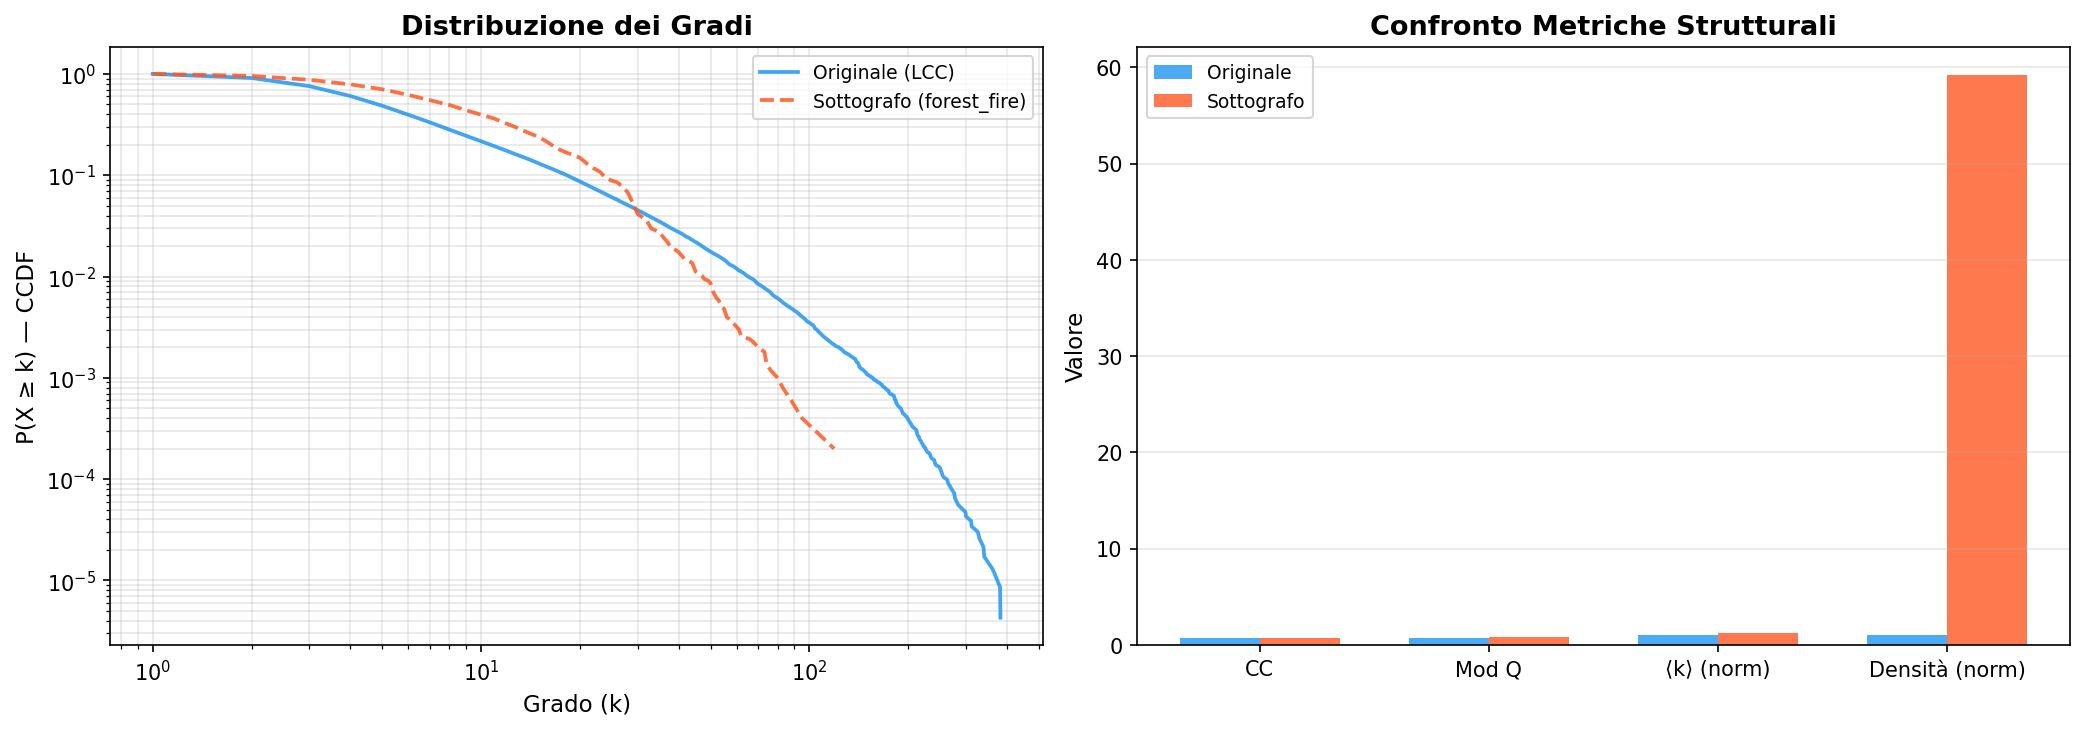
\includegraphics[width=\textwidth]{validazione_strutturale.png}
    \caption{Confronto tra il grafo originale (LCC) e il sottografo campionato tramite Forest Fire Sampling. A sinistra, la distribuzione dei gradi in scala log-log (CCDF), che mostra come il sottografo preservi la forma a legge di potenza tipica delle reti scale-free. A destra, il confronto tra le principali metriche strutturali normalizzate (coefficiente di clustering, modularità, grado medio e densità).}
    \label{fig:validazione-strutturale}
\end{figure}

Il grafico di sinistra riporta la \textit{Complementary Cumulative Distribution Function} (CCDF) del grado dei nodi $P(X \ge k)$ in scala doppiamente logaritmica: l'andamento pressoché lineare di entrambe le curve conferma che sia il grafo originale sia il sottografo seguono una distribuzione dei gradi a coda pesante, coerente con la struttura scale-free attesa per una rete di co-autoraggio accademico. Il grafico di destra confronta invece, in forma normalizzata, il coefficiente di clustering (CC), la modularità (Mod Q), il grado medio $\langle k \rangle$ e la densità: quest'ultima risulta nettamente più alta nel sottografo, come atteso per effetto della riduzione del numero di nodi a parità di connettività locale preservata.

La tabella seguente riporta il confronto quantitativo dettagliato tra le due reti:

\begin{table}[h]
    \centering
    \small
    \begin{tabular}{lrrr}
        \toprule
        \textbf{Metrica} & \textbf{Originale} & \textbf{Sottografo} & \textbf{$\Delta$ relativo} \\
        \midrule
        Nodi                  & 232\,865 & 5\,000  & $-97.9\%$ \\
        Archi                 & 961\,883 & 26\,246 & $-97.3\%$ \\
        Densità               & 0.000035 & 0.002100 & $+5819.6\%$ \\
        Grado medio $\langle k \rangle$ & 8.3    & 10.5    & $+27.1\%$ \\
        Grado max             & 382      & 119     & $-68.8\%$ \\
        $\sigma$(grado)       & 13.4     & 9.7     & $-27.1\%$ \\
        Clustering CC         & 0.7204   & 0.6988  & $-3.0\%$ \\
        Modularity Q          & 0.6957   & 0.8265  & $+18.8\%$ \\
        N. comunità           & 23\,115  & 415     & $-98.2\%$ \\
        \bottomrule
    \end{tabular}
    \caption{Validazione strutturale — confronto tra il grafo originale (LCC) e il sottografo estratto tramite Forest Fire Sampling.}
    \label{tab:validazione-strutturale}
\end{table}

Il rapporto di campionamento risulta pari al 2.1\% dei nodi originali. Dal punto di vista computazionale, il calcolo delle metriche sul grafo completo ha richiesto circa 114 secondi, contro appena 0.4 secondi per il sottografo, con un guadagno di efficienza di oltre due ordini di grandezza. Nel complesso, i valori di clustering e grado medio si mantengono coerenti tra le due reti (scostamenti contenuti entro il $\pm 30\%$), a conferma della bontà del campionamento; l'aumento della modularità nel sottografo ($+18.8\%$) è in parte un effetto atteso della riduzione di scala, che tende a rendere più nette le partizioni in comunità più piccole e numericamente meno frammentate.

\subsubsection{Metriche Baseline del Sottografo}
Una volta completata l'estrazione, il modulo \texttt{metrics} calcola l'intero set di metriche baseline sul sottografo di lavoro (5000 nodi), che costituiscono il punto di riferimento (t=0) rispetto al quale verrà misurata l'evoluzione della rete nelle fasi successive.

\begin{table}[h]
    \centering
    \small
    \begin{tabular}{lr}
        \toprule
        \textbf{Metrica} & \textbf{Valore} \\
        \midrule
        Numero di nodi                     & 5\,000 \\
        Numero di archi                    & 26\,246 \\
        Densità                            & 0.0021 \\
        Grado medio $\langle k \rangle$    & 10.4984 \\
        Componenti connesse                & 1 \\
        Clustering medio                   & 0.6988 \\
        Grado massimo                      & 119 \\
        Grado minimo                       & 1 \\
        $\sigma$(grado)                    & 9.7465 \\
        Modularity Q                       & 0.8265 \\
        Echo Chamber Index (ECI)           & 0.8318 \\
        \bottomrule
    \end{tabular}
    \caption{Metriche strutturali baseline del sottografo (Fase 0, $t=0$).}
    \label{tab:metriche-baseline}
\end{table}

Il grafo risulta composto da un'unica componente connessa, condizione necessaria affinché la diffusione dell'informazione e il rewiring strutturale possano interessare potenzialmente l'intera rete. Il valore di Echo Chamber Index già elevato in partenza (0.8318), in linea con l'alta modularità (0.8265), indica che il sottografo campionato eredita una segregazione comunitaria marcata già nella rete di co-autoraggio originale, ancor prima che il sistema agentico inizi a introdurre dinamiche di polarizzazione.

Il modulo calcola inoltre la classifica dei nodi per PageRank, utilizzata come uno dei criteri di selezione dei pazienti zero nella Fase 1 (Tabella~\ref{tab:top5-pagerank}).

\begin{table}[h]
    \centering
    \small
    \begin{tabular}{clc}
        \toprule
        \textbf{Rank} & \textbf{ID Nodo} & \textbf{PageRank} \\
        \midrule
        1 & 3342 & 0.0011 \\
        2 & 1316 & 0.0009 \\
        3 & 505  & 0.0009 \\
        4 & 3612 & 0.0008 \\
        5 & 863  & 0.0008 \\
        \bottomrule
    \end{tabular}
    \caption{Top-5 nodi per PageRank sul sottografo baseline.}
    \label{tab:top5-pagerank}
\end{table}

\subsection{Fase 1: Livello Cognitivo e Agenti LLM}
Nella Fase 1 si instanziano i processi logici che governano il singolo agente.
\begin{itemize}[leftmargin=*]
    \item \textbf{Inizializzazione Pazienti Zero:} Tramite il modulo \texttt{seeder}, il sistema seleziona 750 nodi (il 15\% della rete) come propagatori iniziali. La selezione avviene tramite una logica \textit{combined} per massimizzare la topologia di diffusione.
    \item \textbf{Orchestrazione Agenti:} A ogni step si attiva il 15\% dei nodi; gli agenti attivi inviano richieste concorrenti (fino a 150 contemporanee, raggruppate in batch dal server vLLM) verso il modello LLM.
    \item \textbf{Generazione di Opinioni:} Gli agenti valutano le proprie metriche, le posizioni dei propri vicini e restituiscono l'opinione testuale che altera il proprio \textit{feature vector}, azionando internamente la macchina a stati.
\end{itemize}

\subsubsection{Approfondimento: i moduli del livello cognitivo}
La Fase 1 si fonda su cinque moduli chiave, che insieme costituiscono il livello cognitivo del sistema: l'agente vero e proprio, il client LLM, il modulo di seeding dei pazienti zero, la macchina a stati e il gestore del grafo dinamico.

\paragraph{agent.py — Agente Cognitivo}
Rappresenta l'entità cognitiva elementare associata a ogni singolo nodo del grafo sociale. Ciascun agente incapsula la memoria, il posizionamento sociale (comunità, centralità) e la logica decisionale guidata da LLM.

\begin{itemize}[leftmargin=*]
    \item \textbf{Ciclo di vita del singolo step:}
    \begin{enumerate}
        \item \textit{Percezione} (\texttt{prepare\_step}): interroga il \texttt{NetworkManager} per estrarre la cronologia recente dei post pubblicati dai suoi contatti (feed) e calcolare la distribuzione degli stati del vicinato.
        \item \textit{Cognizione} (\texttt{cognize}): prepara i prompt di sistema e utente strutturati e invia la richiesta al modulo \texttt{LLMClient}, ottenendo un output JSON standardizzato.
        \item \textit{Azione e transizione} (\texttt{finalize\_step}): esegue il parsing del JSON (estraendo opinione testuale, livello di suscettibilità e intenzione di condivisione); se lo desidera, l'agente pubblica un post, calcola la perturbazione vettoriale dell'embedding del nodo e aggiorna lo stato discreto consultando la macchina a stati.
    \end{enumerate}
    \item \textbf{Perturbazione degli embedding:} le transizioni di stato spostano l'embedding del nodo lungo una direzione ``ideologica'' comune a tutta la rete: gli Infetti in un verso, Resistenti e Fact-Checker nel verso opposto, con una piccola componente individuale (10\%). In questo modo la similarità tra embedding, e quindi la link prediction della GNN, riflette la vicinanza di opinione tra agenti.
    \item \textbf{Ottimizzazioni per grandi grafi:}
    \begin{itemize}
        \item \textit{Fast Path Optimization}: se l'agente è Suscettibile (S) e non ha alcun vicino infetto o fact-checker adiacente, la chiamata all'LLM e la costruzione del prompt vengono del tutto saltate, poiché non riceve alcuna pressione di diffusione e rimarrebbe stabile in S.
        \item \textit{Smart Cache}: se lo stato e il feed del vicinato sono identici allo step precedente, riutilizza la risposta LLM in memoria senza inviare una nuova richiesta di rete.
    \end{itemize}
\end{itemize}

\paragraph{llm\_client.py — Wrapper LLM Portabile}
Gestisce la comunicazione diretta con i modelli di linguaggio (le API cloud di Gemini o i server di inferenza locali compatibili con OpenAI, quali Ollama e vLLM) in modo robusto e protetto.

\begin{itemize}[leftmargin=*]
    \item \textbf{Funzionalità di rete:} implementa retry automatici con backoff esponenziale per gestire disconnessioni temporanee o limiti di rate-limiting API, e pulisce/valida l'output testuale per garantire la corretta decodifica in formato JSON.
    \item \textbf{Riproducibilità:} ogni richiesta porta un seed derivato dal contenuto del prompt, così che due run che ricevono lo stesso prompt ottengano la stessa risposta. È la condizione che rende confrontabili la run con intervento e quella di controllo della Fase 3.
    \item \textbf{Caching su disco} (\texttt{LLMDiskCache}): salva le risposte LLM su file JSONL persistente in modo thread-safe. Se la simulazione viene interrotta a metà (ad esempio superando il limite di tempo su Kaggle), al riavvio riutilizza le risposte già registrate per non perdere progresso.
    \item \textbf{Controllo dei costi} (\texttt{TokenBudget}): un singleton globale che accumula ad ogni chiamata il consumo di token (sia in input che in output), dotato di una soglia di avviso (\texttt{warn\_at}) e di una soglia di arresto forzato (\texttt{hard\_limit}) per prevenire addebiti monetari indesiderati sulle API.
\end{itemize}

\paragraph{seeder.py — Seeding dei Pazienti Zero}
Si occupa di individuare e infettare i nodi iniziali (``Pazienti Zero'', stato I) per innescare e far propagare la narrazione polarizzante all'interno del sottografo.

\begin{itemize}[leftmargin=*]
    \item \textbf{Strategie di selezione} (\texttt{select}):
    \begin{itemize}
        \item \textit{pagerank/degree/katz/betweenness}: seleziona i top-$k$ nodi aventi rispettivamente i punteggi più alti per queste metriche (influencer globali, ponti strutturali o hub locali).
        \item \textit{combined} (default): assegna a ogni nodo uno score pesato normalizzato (40\% PageRank, 40\% Katz, 20\% Degree) per identificare i nodi con il massimo potenziale di impatto locale e globale.
        \item \textit{cross\_community}: ripartisce i semi equamente tra tutte le comunità Louvain rilevate, selezionando il nodo con lo score combinato più alto all'interno di ciascuna, per coprire uniformemente il grafo.
        \item \textit{random}: selezione casuale riproducibile tramite seed.
    \end{itemize}
    \item \textbf{Iniezione} (\texttt{inject}): forza lo stato iniziale dei nodi selezionati a I (Infected) e forza la pubblicazione del primo post di propaganda per attivare il feed dei rispettivi vicini.
\end{itemize}

\paragraph{state\_machine.py — Macchina a Stati}
Governa le transizioni di stato discrete degli agenti (S $\to$ Suscettibile, I $\to$ Infetto, R $\to$ Resistente, F $\to$ Fact-Checker) implementando un modello Linear Threshold (LT) esteso.

\begin{itemize}[leftmargin=*]
    \item \textbf{Soglie individuali:} ogni nodo $u$ ha una soglia $\theta_u$ che dipende soltanto dal seed globale e dall'identificativo del nodo. La soglia è quindi identica in ogni sessione e dopo ogni ripresa da checkpoint, indipendentemente dall'ordine in cui i nodi vengono interrogati.
    \item \textbf{Modulazione cognitiva delle soglie:} nei modelli classici LT, un nodo si infetta se la frazione di vicini infetti supera una soglia fissa $\theta_u$. Qui la soglia è riscalata in base all'output qualitativo dell'agente LLM:
    \[
        \theta_{\text{eff}} = \theta_u \times (1.5 - \text{susceptibility})
    \]
    Se l'agente dichiara alta suscettibilità, la sua soglia scende, rendendolo più vulnerabile all'influenza dei vicini.
    \item \textbf{Regole di transizione principali:}
    \begin{itemize}
        \item \textit{S $\to$ I}: avviene se la pressione del vicinato supera la soglia efficace ($\text{fraction\_I} \ge \theta_{\text{eff}}$) \textbf{e} l'agente stesso propone il cambio di stato nel JSON.
        \item \textit{S $\to$ R} (resistenza spontanea): avviene se l'agente, esposto all'infezione (almeno il 12\% di vicini infetti), ha bassa suscettibilità e rifiuta la condivisione.
        \item \textit{S $\to$ R} (inoculazione): avviene se la frazione di vicini Fact-Checker raggiunge \texttt{fc\_protection\_threshold} (0.10), non è inferiore alla frazione di vicini infetti e l'agente non propone di passare a I.
        \item \textit{I $\to$ R}: avviene se la frazione di vicini Fact-Checker raggiunge \texttt{fc\_resistance\_threshold} (0.25) oppure se l'agente corregge autonomamente la sua visione.
        \item \textit{R $\to$ I} (Ricaduta): possibile ma molto rara, innescata solo con almeno il 60\% di vicini infetti e una suscettibilità cognitiva molto alta ($>0.8$).
    \end{itemize}
\end{itemize}

\paragraph{network\_manager.py — Gestore del Grafo}
Funge da unico layer di astrazione e persistenza per la rete sociale dinamica. Qualsiasi modulo esterno che desideri interrogare o alterare la struttura del grafo deve transitare per il \texttt{NetworkManager}.

\begin{itemize}[leftmargin=*]
    \item \textbf{Post Store:} memorizza la lista di post scritti da ciascun nodo e costruisce la vista del feed per gli adiacenti (\texttt{get\_feed}), ordinandoli in modo decrescente per step temporale.
    \item \textbf{Topologia e rewiring:} aggiunge archi (\texttt{add\_edge}), rimuove archi (\texttt{remove\_edge}) e gestisce le transizioni strutturali in blocco (\texttt{apply\_rewiring}) calcolate dalla GNN.
    \item \textbf{Gestione vettoriale:} custodisce la matrice degli embedding dei nodi, che vengono perturbati dagli agenti ad ogni iterazione fornendo il segnale dinamico su cui lavora la GNN; consente aggiornamenti massivi ottimizzati (\texttt{perturb\_embeddings\_batch}).
    \item \textbf{Codifica delle opinioni:} espone un'unica codifica numerica degli stati (\texttt{STATE\_TO\_BELIEF}: S $= 0$, I $= +1$, R $=$ F $= -1$), usata da tutte le metriche di opinione.
    \item \textbf{Checkpointing:} salva (\texttt{save}) e ripristina (\texttt{load}) lo stato completo della simulazione (grafo NetworkX, post, stati ideologici e matrice degli embedding) su file pickle.
\end{itemize}

\subsection{Fase 2: Dinamiche di Rete e Co-evoluzione}
La Fase 2 innesca il ciclo ricorsivo vero e proprio, supervisionato dal \texttt{SimulationOrchestrator}.
\begin{itemize}[leftmargin=*]
    \item \textbf{Graph Rewiring (GNN):} La GNN elabora i feature vector alterati dagli agenti. Attraverso il modulo \texttt{rewirer}, la rete subisce variazioni dinamiche a densità costante: ogni nuovo arco tra agenti con score di link prediction elevato sostituisce l'arco esistente con lo score più basso. Il rewiring avviene con un intervallo di \textit{cooldown} di 2 step e sostituisce al massimo 50 archi per volta.
    \item \textbf{Transizione e Contagio:} Contemporaneamente alla GNN, si verifica un aggiornamento degli stati via \textit{Linear Threshold}. A ogni step il 15\% dei nodi della rete valuta l'influenza cumulativa del vicinato e si adegua se la pressione sociale supera la propria resistenza individuale.
    \item \textbf{Checkpointing Resiliente:} L'Orchestratore compie frequenti backup di stato su file serializzati (\texttt{.pkl}) e in \texttt{metrics\_history.csv}. Il sistema ripristina il \textit{loop} dal checkpoint più recente per superare i vincoli temporali dell'ambiente cloud, agganciando i log pregressi alle nuove run; se il percorso indicato non esiste, il notebook cerca automaticamente checkpoint e CSV tra i dati in input della sessione Kaggle.
\end{itemize}

\subsubsection{Approfondimento: orchestrator.py — Il Motore Centrale}
Il modulo \texttt{orchestrator.py} definisce la classe \texttt{SimulationOrchestrator}, che rappresenta il motore centrale del framework. Ha il compito di coordinare tutte le fasi del loop co-evolutivo a ogni step temporale, gestire il checkpointing/resume e far comunicare i vari sottosistemi (grafi, agenti LLM e GNN).

\paragraph{Inizializzazione (\texttt{build\_from\_config})}
Costruisce la simulazione partendo dall'oggetto \texttt{Config}, seguendo una sequenza precisa:
\begin{enumerate}
    \item imposta i seed globali per la riproducibilità;
    \item carica il sottografo campionato e le comunità;
    \item inizializza gli embedding dei nodi (Word2Vec);
    \item istanzia il \texttt{NetworkManager} come unica sorgente di verità;
    \item calcola le centralità e usa il \texttt{Seeder} per infettare i pazienti zero iniziali;
    \item ripristina lo stato precedente (Resume) se rileva checkpoint validi su disco, insieme a mappa delle comunità e metriche cumulative;
    \item instanzia gli \texttt{Agent}, leggendo lo stato effettivo di ciascun nodo dal grafo ripristinato, e i relativi client LLM;
    \item crea il modello \texttt{GraphSAGEModel}, il \texttt{GNNTrainer} e il \texttt{Rewirer}.
\end{enumerate}

\paragraph{Il loop principale (\texttt{run} e \texttt{\_run\_step})}
Il metodo \texttt{run} esegue un ciclo temporale per $N$ passi, ripartendo dallo step successivo all'ultimo completato. A ogni singolo step \texttt{\_run\_step(t)}, l'orchestratore esegue in sequenza i tre cicli interni descritti di seguito, calcola le metriche aggregate, salva lo stato nel log JSONL e nel CSV, e scrive un checkpoint periodico.

\paragraph{I tre cicli interni dell'Orchestratore}
\begin{itemize}[leftmargin=*]
    \item \textbf{Ciclo Agenti} (\texttt{\_agent\_cycle}): è il ciclo più critico a livello prestazionale a causa delle chiamate LLM (latenza di inferenza). Per risolverlo, l'Orchestratore implementa un design a tre fasi:
    \begin{enumerate}
        \item \textit{PREPARE} (sequenziale): legge in memoria dal \texttt{NetworkManager} e costruisce i messaggi di prompt per l'LLM di ogni nodo; fase puramente in memoria, richiede frazioni di secondo.
        \item \textit{DISPATCH} (parallela): invia le richieste \texttt{llm.chat()} dei nodi in parallelo tramite un thread pool (\texttt{ThreadPoolExecutor}), nascondendo la latenza di I/O; i nodi inattivi vengono saltati grazie alla Fast Path Optimization e alla Smart Cache. Se fallisce più del 50\% delle chiamate (\texttt{max\_llm\_failure\_rate}), lo step viene interrotto prima di modificare lo stato della rete, e l'ultimo checkpoint resta valido.
        \item \textit{FINALIZE} (sequenziale): riceve i risultati dell'LLM, esegue il parsing del JSON, valuta il cambio di stato tramite \texttt{StateMachine} ed esprime l'opinione nel post.
    \end{enumerate}
    Come ottimizzazione, invece di aggiornare l'embedding nodo per nodo, il ciclo raccoglie tutti i delta di perturbazione e li applica alla fine in un'unica operazione vettorizzata tramite \texttt{perturb\_embeddings\_batch}.
    \item \textbf{Ciclo GNN} (\texttt{\_gnn\_cycle}): preleva la matrice degli embedding dei nodi aggiornata dagli agenti, esegue un passo di addestramento (\texttt{GNNTrainer.train\_step}) sul grafo corrente per allineare la rete neurale alle nuove posizioni ideologiche dei nodi, ed estrae le predizioni di link prediction (\texttt{predict\_links}) sulle coppie candidate. I candidati sono coppie a distanza 2 generate a partire da 500 nodi sorgente, al massimo 5 per sorgente; le sorgenti cambiano a ogni step, così che il rewiring esplori nel tempo l'intera rete.
    \item \textbf{Ciclo di Rewiring} (\texttt{\_rewiring\_cycle}): ad ogni intervallo di cooldown, interroga il \texttt{Rewirer} fornendogli i punteggi predetti dalla GNN e gli stati correnti degli agenti. In modalità \texttt{swap} (default) il \texttt{Rewirer} abbina ogni arco da aggiungere (nuovo legame omofilo) alla rimozione dell'arco esistente con lo score più basso, mantenendo costante la densità; un vincolo di sicurezza impedisce di isolare un nodo, tenendo conto anche delle rimozioni già decise nello stesso step. I cambiamenti vengono comunicati al \texttt{NetworkManager} per mutare la topologia fisica del grafo.
\end{itemize}

\paragraph{Moduli richiamati dall'Orchestratore}
L'Orchestratore unifica e richiama moduli provenienti da quattro diversi sottosistemi:
\begin{itemize}[leftmargin=*]
    \item \textbf{Sottosistema \texttt{graph}} (gestione rete e metriche): \texttt{network\_manager.py} (\texttt{NetworkManager}), che custodisce la topologia fisica, i post e gli embedding, gestendo le transizioni topologiche del rewiring; \texttt{metrics.py} (\texttt{compute\_centralities}, \texttt{compute\_all\_metrics}), che calcola l'importanza dei nodi all'avvio e, alla fine di ogni step, le metriche strutturali (modularità, Echo Chamber Index) e di opinione (omofilia, assortatività, polarizzazione).
    \item \textbf{Sottosistema \texttt{agents}} (logica cognitiva degli autori): \texttt{agent.py} (\texttt{Agent}, \texttt{AgentStepContext}), che incapsula il comportamento decisionale dell'agente; \texttt{seeder.py} (\texttt{Seeder}), che trova i nodi hub iniziali per l'iniezione dei semi ideologici; \texttt{state\_machine.py} (\texttt{StateMachine}), che calcola la transizione Linear Threshold modulata dalla suscettibilità dell'utente; \texttt{llm\_client.py} (\texttt{LLMClient}, \texttt{MockLLMClient}), interfaccia per le chiamate al modello o al mock usato nei test.
    \item \textbf{Sottosistema \texttt{gnn}} (rappresentazione e link prediction): \texttt{embeddings.py} (\texttt{EmbeddingManager}), che carica ed esporta la matrice di embedding Word2Vec; \texttt{model.py} (\texttt{GraphSAGEModel}), il modello GraphSAGE implementato in PyTorch Geometric (o NumPy per fallback); \texttt{trainer.py} (\texttt{GNNTrainer}), che gestisce il loop di ottimizzazione e predice i link candidati per il rewiring; \texttt{rewirer.py} (\texttt{Rewirer}), che seleziona gli archi da aggiungere e da rimuovere a partire dagli score della GNN.
    \item \textbf{Sottosistema \texttt{utils}} (log, checkpoint e determinismo): \texttt{logger.py} (\texttt{SimLogger}), che scrive lo storico delle metriche e transizioni in formato JSONL; \texttt{checkpoint.py} (\texttt{CheckpointManager}), che serializza e deserializza lo stato completo del framework ad intervalli regolari, ordinando e potando i checkpoint per numero di step; \texttt{seed.py} (\texttt{set\_all\_seeds}), che imposta i seed casuali per garantire la riproducibilità degli esperimenti.
\end{itemize}

\subsubsection{Dinamiche Osservate in Fase 2}
L'esecuzione documentata usa l'LLM reale in tutte le fasi. La Fase 2 comprende 100 step (0--99), eseguiti in due sessioni Kaggle da 50 step ciascuna con ripresa da checkpoint. Il file \texttt{metrics\_history.csv} registra l'evoluzione dello stato della rete ad ogni step.

\begin{figure}[h]
    \centering
    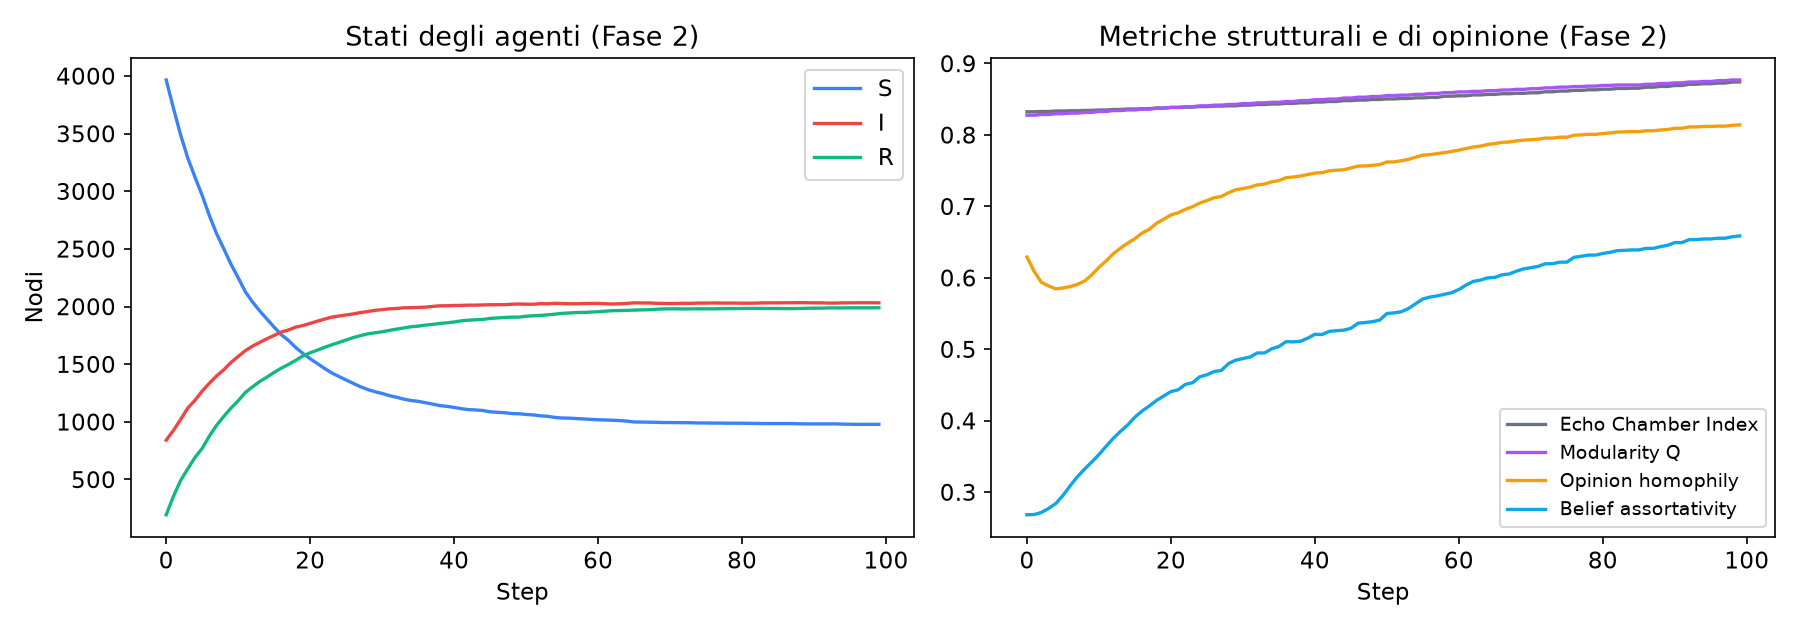
\includegraphics[width=\textwidth]{fase2_dinamiche.png}
    \caption{Evoluzione della rete durante la Fase 2 (step 0--99). A sinistra, la dinamica delle popolazioni di agenti negli stati S (Suscettibile), I (Infetto) e R (Resistente). A destra, l'evoluzione delle metriche strutturali (Echo Chamber Index, Modularity Q) e di opinione (Opinion homophily, Belief assortativity).}
    \label{fig:fase2-dinamiche}
\end{figure}

\begin{table}[h]
    \centering
    \small
    \begin{tabular}{rrrrrrrr}
        \toprule
        \textbf{Step} & \textbf{S} & \textbf{I} & \textbf{R} & \textbf{ECI} & \textbf{Mod. Q} & \textbf{Op. homophily} & \textbf{Belief assort.} \\
        \midrule
        0  & 3\,965 & 841    & 194    & 0.832 & 0.828 & 0.629 & 0.268 \\
        25 & 1\,363 & 1\,927 & 1\,710 & 0.840 & 0.841 & 0.708 & 0.464 \\
        49 & 1\,070 & 2\,022 & 1\,908 & 0.850 & 0.854 & 0.759 & 0.541 \\
        75 & 990    & 2\,030 & 1\,980 & 0.861 & 0.867 & 0.797 & 0.622 \\
        99 & 978    & 2\,032 & 1\,990 & 0.874 & 0.877 & 0.814 & 0.659 \\
        \bottomrule
    \end{tabular}
    \caption{Andamento della Fase 2 a intervalli di circa 25 step.}
    \label{tab:fase2}
\end{table}

Il grafico di sinistra mostra un tipico andamento epidemico. La popolazione Suscettibile decresce da 3\,965 a 978 unità; gli Infetti superano i Suscettibili già allo step 16, crescono rapidamente nei primi 30 step e poi si stabilizzano intorno al 41\% dei nodi (picco di 2\,034 infetti allo step 88). I Resistenti crescono con lo stesso andamento ma restano sempre leggermente sotto gli Infetti (1\,990 contro 2\,032 allo step 99).

Il grafico di destra mette a confronto due letture della segregazione, che in questa run crescono entrambe. Le metriche strutturali salgono in modo graduale e regolare: la modularità passa da 0.828 a 0.877 e l'Echo Chamber Index da 0.832 a 0.874. Le metriche di opinione crescono in modo molto più marcato: la belief assortativity sale da 0.27 a 0.66 (circa due volte e mezzo) e l'opinion homophily da 0.63 a 0.81, dopo un calo iniziale nei primi 4 step dovuto alla prima ondata di contagio. Il rewiring guidato dalla GNN rafforza quindi le community esistenti della rete di co-autoraggio e, in misura maggiore, raggruppa i nodi che condividono la stessa opinione.

Il rewiring sostituisce complessivamente 2\,500 archi in 100 step, circa il 10\% della rete, a densità costante (26\,246 archi). Alla fine della Fase 2 la rete conta 86 componenti connesse invece di una: il vincolo di sicurezza impedisce di isolare singoli nodi, ma il rewiring può staccare piccoli gruppi dal resto della rete.

\subsection{Fase 3: Intervento e Fact-Checking}
L'ultima fase simula una contromisura strategica contro la diffusione della narrazione polarizzante.
\begin{itemize}[leftmargin=*]
    \item \textbf{Influence Maximization:} Il modulo d'intervento individua un set limitato di nodi (parametro \texttt{CELF\_BUDGET\_K = 20}) ideali per una campagna di contrasto, massimizzando il numero di agenti su cui la pressione dei fact-checker sarà sufficiente a produrre una transizione.
    \item \textbf{Azione sui vicini:} I \textit{fact-checker} pubblicano contenuti correttivi nei feed dei vicini e, attraverso le soglie della macchina a stati, possono rendere resistenti sia i Suscettibili (inoculazione) sia gli Infetti.
\end{itemize}

La Fase 3 — \textit{Deployment \& Fact-Checking} — ha lo scopo di valutare l'efficacia delle strategie di contrasto alla disinformazione all'interno della rete sociale simulata. Introduce un sottoinsieme di agenti con il ruolo di Fact-Checker (stato F), con l'obiettivo di frenare l'infezione della narrazione polarizzante e spingere gli agenti infetti (I) o suscettibili (S) a diventare resistenti (R).

\paragraph{Disegno sperimentale: intervento e controllo.} Un semplice confronto ``prima/dopo'' su una sola run mescolerebbe l'effetto dei fact-checker con l'evoluzione spontanea della rete, che continua a cambiare anche senza intervento. Per isolare l'effetto, la Fase 3 viene eseguita due volte a partire dallo stesso checkpoint di fine Fase 2 e per lo stesso numero di step: una run con l'iniezione dei fact-checker e una run di controllo senza (\texttt{CONTROL\_RUN = True} nel notebook). Grazie al seed per richiesta dell'LLM, le due run ricevono le stesse risposte finché i prompt coincidono. L'effetto dell'intervento è la differenza tra le due run allo stesso step.

\subsubsection{Il Flusso di Esecuzione della Fase 3}
Il processo si sviluppa attraverso sette passaggi logici:
\begin{enumerate}
    \item \textbf{Ripristino dello stato:} il notebook inizializza il \texttt{CheckpointManager} e l'orchestratore \texttt{SimulationOrchestrator} per ricaricare l'ultimo checkpoint salvato al termine della Fase 2 (co-evoluzione).
    \item \textbf{Calcolo della baseline pre-intervento:} vengono calcolate le metriche strutturali e di opinione correnti (Infection Rate, modularità Q, Echo Chamber Index, polarizzazione, omofilia e assortatività delle opinioni) per registrare lo stato della rete prima dell'iniezione.
    \item \textbf{Verifica della soglia e selezione dei seed:} l'intervento si attiva se l'infection rate supera \texttt{activation\_threshold} (0.4); il parametro \texttt{FORCE\_INJECTION} consente di iniettare comunque, registrandolo nel report. Vengono poi selezionati i $k$ nodi in cui posizionare i fact-checker. Nella run di controllo questo passaggio e il successivo vengono saltati.
    \item \textbf{Iniezione dei fact-checker:} la classe \texttt{FactCheckerInjector} converte lo stato dei nodi selezionati in F e vi inserisce un post iniziale di fact-checking per attivare la propagazione nei feed dei rispettivi vicini; lo stato degli agenti viene poi sincronizzato con il grafo (\texttt{sync\_agent\_states}).
    \item \textbf{Simulazione post-intervento:} l'orchestratore fa avanzare la simulazione per $N$ step post-intervento, ripartendo dallo step successivo all'ultimo della Fase 2. Durante questa fase gli agenti vicini ai nodi F leggono i post correttivi e, in base alle soglie e al loro livello cognitivo di suscettibilità, possono transitare in R. Gli step vengono eseguiti dalla stessa istanza dell'\texttt{SimulationOrchestrator}, con lo stesso LLM reale (server vLLM locale) impiegato nelle fasi precedenti.
    \item \textbf{Confronto delle metriche:} viene calcolato il report finale con le metriche di fine run, le metriche dei fact-checker e le variazioni rispetto alla baseline pre-intervento.
    \item \textbf{Salvataggio del report:} tutti i dati dell'intervento (inclusi i node ID scelti e la stima dei nodi coperti) vengono scritti in \texttt{results/phase3\_report.json}, oppure in \texttt{results/phase3\_report\_control.json} per la run di controllo. L'ultima cella del notebook (\textit{Confronto Intervento vs Controllo}) confronta infine le due run, usando solo i report con il flag \texttt{control\_run} atteso e almeno uno step di Fase 3, e salva l'effetto dell'intervento in \texttt{results/phase3\_comparison.json}.
\end{enumerate}

\subsubsection{Moduli Richiamati nella Fase 3}
La Fase 3 si appoggia sul sottosistema di mitigazione dell'influenza ideologica (\texttt{src/influence/}) e riutilizza in modo coordinato i moduli precedentemente presentati.

\paragraph{Sottosistema \texttt{src/influence/} — Algoritmi e Valutazione}
\begin{itemize}[leftmargin=*]
    \item \textbf{celf.py} (selezione dei seed): esclude dal pool degli eleggibili i nodi già Infetti (I), già Fact-Checker (F) o già Resistenti (R) — iniettare un fact-checker su un nodo già resistente sarebbe uno spreco di budget. Supporta due obiettivi:
    \begin{itemize}
        \item \texttt{threshold} (default): conta i nodi su cui la pressione dei fact-checker supera le stesse soglie che nella simulazione producono una transizione (S $\to$ R con almeno il 10\% di vicini F, I $\to$ R con almeno il 25\%). Il calcolo è deterministico ed esatto. Poiché una funzione a soglia non è submodulare, non si usa la valutazione lazy di CELF ma il greedy completo, il cui costo è comunque trascurabile.
        \item \texttt{ic}: algoritmo CELF (\textit{Cost-Effective Lazy Forward}) su modello Independent Cascade, con stime Monte Carlo (30 round) su numeri casuali comuni a tutti i candidati e guadagni marginali troncati a zero; le simulazioni sfruttano il parallelismo su CPU (\texttt{ProcessPoolExecutor}).
    \end{itemize}
    \item \textbf{injector.py} (\texttt{FactCheckerInjector}): gestisce la logica di attivazione (\texttt{should\_activate}, che fa scattare l'intervento solo se l'infection rate supera la soglia critica \texttt{activation\_threshold}) e inietta lo stato F nei nodi seed selezionati. Forza la pubblicazione di un post di fact-checking iniziale nel \texttt{NetworkManager} (del tipo \textit{``[FACT-CHECK seed] I have been designated to critically examine claims about `[Topic]'\ldots''}), che funge da scintilla per la diffusione dell'informazione correttiva nei feed dei nodi adiacenti.
    \item \textbf{metrics.py} (metriche di influenza):
    \begin{itemize}
        \item \textit{Reach dei fact-checker} (\texttt{compute\_fact\_checker\_spread}): numero di nodi entro \texttt{reach\_hops} salti (default 1) da almeno un nodo F, cioè la platea che vede direttamente i contenuti correttivi.
        \item \textit{Copertura efficace} (\texttt{fc\_effective\_coverage}): frazione di nodi su cui la pressione dei fact-checker supera le soglie di transizione, cioè quelli che l'intervento può effettivamente convertire.
        \item \textit{Intervention Delta} (\texttt{compute\_intervention\_delta}): differenze (dopo $-$ prima) delle metriche rispetto alla baseline pre-intervento.
    \end{itemize}
\end{itemize}

\paragraph{Altri Sottosistemi Richiamati}
\begin{itemize}[leftmargin=*]
    \item \textbf{orchestrator.py} (\texttt{SimulationOrchestrator}): coordina l'evoluzione del sistema negli step successivi all'iniezione dei fact-checker, aggiornando post, stati cognitivi e il rewiring della GNN; è la stessa istanza dell'orchestratore costruita per le Fasi 1 e 2 (parametro \texttt{USE\_MOCK\_LLM = False} nel notebook), per cui gli agenti continuano a interrogare l'LLM reale anche durante il post-intervento.
    \item \textbf{network\_manager.py} (\texttt{NetworkManager}): riceve i post di fact-checking dei seed e si assicura che vengano propagati nei feed degli agenti vicini.
    \item \textbf{metrics.py} (\texttt{compute\_all\_metrics}): calcola le metriche strutturali e di opinione all'inizio (baseline) e alla fine del post-intervento.
    \item \textbf{checkpoint.py} (\texttt{CheckpointManager}): fornisce i dati di ripristino per caricare la rete al termine della Fase 2 e avviare entrambi gli scenari della Fase 3.
\end{itemize}

\subsubsection{Risultati: Intervento a Confronto con il Controllo}
Entrambe le run partono dal checkpoint dello step 99 ed eseguono 30 step post-intervento (step 100--129), con \texttt{CELF\_BUDGET\_K = 20}. L'intervento è partito con un infection rate di 0.406, sopra la soglia di attivazione (0.4), quindi senza forzature. La selezione con obiettivo \texttt{threshold} ha scelto 20 nodi suscettibili, con una stima di 162 nodi coperti.

\begin{table}[h]
    \centering
    \small
    \begin{tabular}{lrrr}
        \toprule
        \textbf{Metrica (step 129)} & \textbf{Con fact-checker} & \textbf{Controllo} & \textbf{Effetto} \\
        \midrule
        Nodi S               & 798    & 974    & $-176$ (di cui 20 seed divenuti F) \\
        Nodi I               & 2\,020 & 2\,024 & $-4$ \\
        Nodi R               & 2\,162 & 2\,002 & $+160$ \\
        Infection Rate       & 0.404  & 0.405  & $-0.001$ \\
        Belief Assortativity & 0.704  & 0.692  & $+0.012$ \\
        Opinion Homophily    & 0.831  & 0.831  & $0.000$ \\
        Belief Polarisation  & 0.839  & 0.805  & $+0.034$ \\
        Echo Chamber Index   & 0.886  & 0.886  & $0.000$ \\
        Modularity Q         & 0.883  & 0.884  & $0.000$ \\
        Transizioni in 30 step & 177  & 17     & $+160$ \\
        \bottomrule
    \end{tabular}
    \caption{Effetto dell'intervento allo step 129: run con 20 fact-checker a confronto con la run di controllo partita dallo stesso checkpoint.}
    \label{tab:intervento-controllo}
\end{table}

\begin{figure}[h]
    \centering
    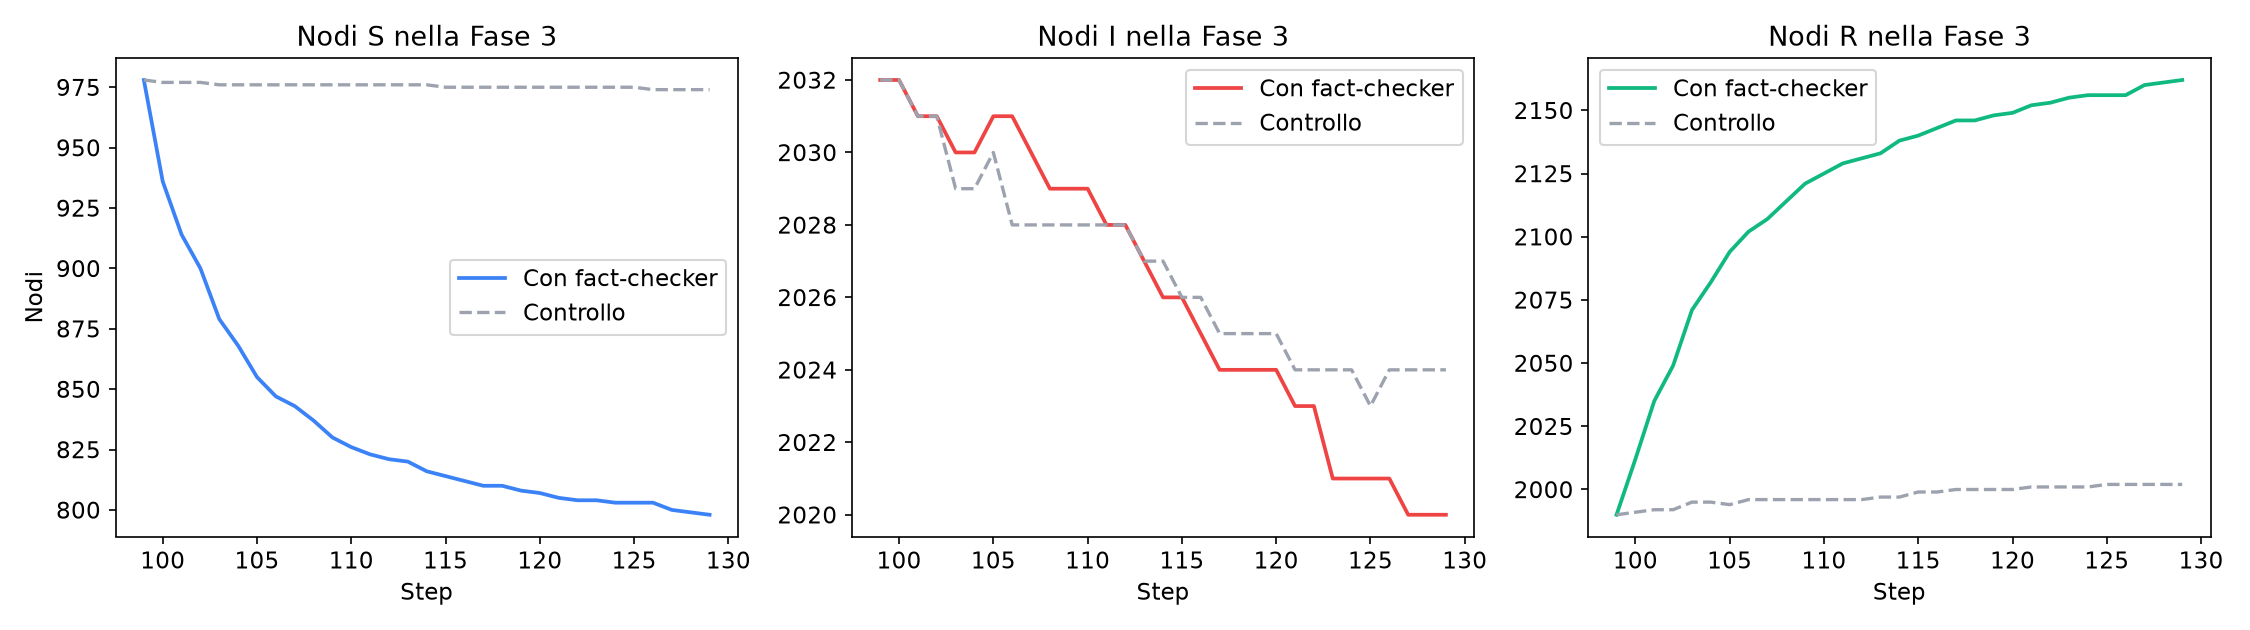
\includegraphics[width=\textwidth]{fase3_confronto.png}
    \caption{Evoluzione dei nodi Suscettibili (sinistra), Infetti (centro) e Resistenti (destra) dallo step 99 allo step 129, nella run con fact-checker (linea continua) e nella run di controllo (linea tratteggiata). Le scale verticali sono diverse: la variazione degli Infetti è di pochi nodi.}
    \label{fig:fase3-confronto}
\end{figure}

\begin{table}[h]
    \centering
    \small
    \begin{tabular}{rrrrr}
        \toprule
        \textbf{Step} & \textbf{S (FC)} & \textbf{S (controllo)} & \textbf{I (FC)} & \textbf{I (controllo)} \\
        \midrule
        99  & 978 & 978 & 2\,032 & 2\,032 \\
        100 & 936 & 977 & 2\,032 & 2\,032 \\
        105 & 855 & 976 & 2\,031 & 2\,030 \\
        110 & 826 & 976 & 2\,029 & 2\,028 \\
        120 & 807 & 975 & 2\,024 & 2\,025 \\
        129 & 798 & 974 & 2\,020 & 2\,024 \\
        \bottomrule
    \end{tabular}
    \caption{Andamento di Suscettibili e Infetti nelle due run (FC = run con fact-checker).}
    \label{tab:fase3-andamento}
\end{table}

Alla fine della run, i 20 fact-checker raggiungono direttamente 194 nodi (9.7 per fact-checker in media), mentre i nodi su cui la loro pressione supera ancora le soglie di transizione sono soltanto 5 (copertura efficace dello 0.10\%): gran parte dei vicini raggiungibili è già stata convertita nei primi step.

\subsubsection{Conclusioni sull'Efficacia dell'Intervento}
Il confronto con il controllo restituisce un quadro netto su un fronte e più sfumato sugli altri.

\begin{itemize}[leftmargin=*]
    \item \textbf{Protezione dei suscettibili:} è l'effetto principale. I fact-checker convertono in resistenti 156 suscettibili in più rispetto al controllo (176 meno i 20 seed), quasi tutti nei primi 10 step: 135 delle 177 transizioni avvengono negli step 100--109, con 14--23 transizioni per step all'inizio e 0--4 alla fine. La stima della selezione (162 nodi coperti) coincide quasi esattamente con i resistenti in più rispetto al controllo ($+160$).
    \item \textbf{Infetti:} l'effetto è trascurabile, perché un infetto si converte solo se almeno un quarto dei suoi vicini è fact-checker. Gli infetti calano di poco in entrambe le run (da 2\,032 a 2\,020 con i fact-checker, a 2\,024 nel controllo): la differenza finale di $-4$ nodi si forma solo negli ultimi 15 step e non è distinguibile dalla variabilità della singola run.
    \item \textbf{Echo chamber:} l'intervento non le riduce e anzi aumenta leggermente la belief assortativity ($+0.012$). I nodi protetti diventano resistenti accanto ad altri resistenti, rafforzando i gruppi di opinione esistenti. Anche la polarizzazione cresce ($+0.034$), perché nodi neutrali (S) passano a una posizione netta (R).
    \item \textbf{Struttura:} Echo Chamber Index e modularità sono praticamente uguali nelle due run. L'intervento agisce sulle opinioni, non sulla topologia della rete.
    \item \textbf{Sproporzione tra budget e scala della rete:} 20 fact-checker rappresentano lo 0.4\% della popolazione, introdotti quando gli infetti sono già oltre 2\,000 e la loro crescita si è stabilizzata. Con le regole del modello, un budget così ridotto e tardivo può proteggere chi non è ancora stato contagiato, ma non recuperare una popolazione infetta già consolidata.
\end{itemize}

L'effetto sui suscettibili è netto. Quelli sugli infetti e sull'assortatività sono piccoli: poiché ogni configurazione è stata eseguita una sola volta, vanno letti con cautela e andrebbero confermati con più repliche.

% ==========================================
% SEZIONE 4: CONCLUSIONI
% ==========================================
\section{Conclusioni e Prospettive}

\subsection{Visualizzazione della Rete: Topologia Iniziale vs Finale}
A completamento dell'analisi quantitativa, è utile osservare direttamente l'evoluzione strutturale della rete attraverso un confronto visivo tra la topologia allo step 0 e quella al termine della simulazione (step 129), su un campione di 150 nodi centrati sugli hub principali del grafo.

\begin{figure}[h]
    \centering
    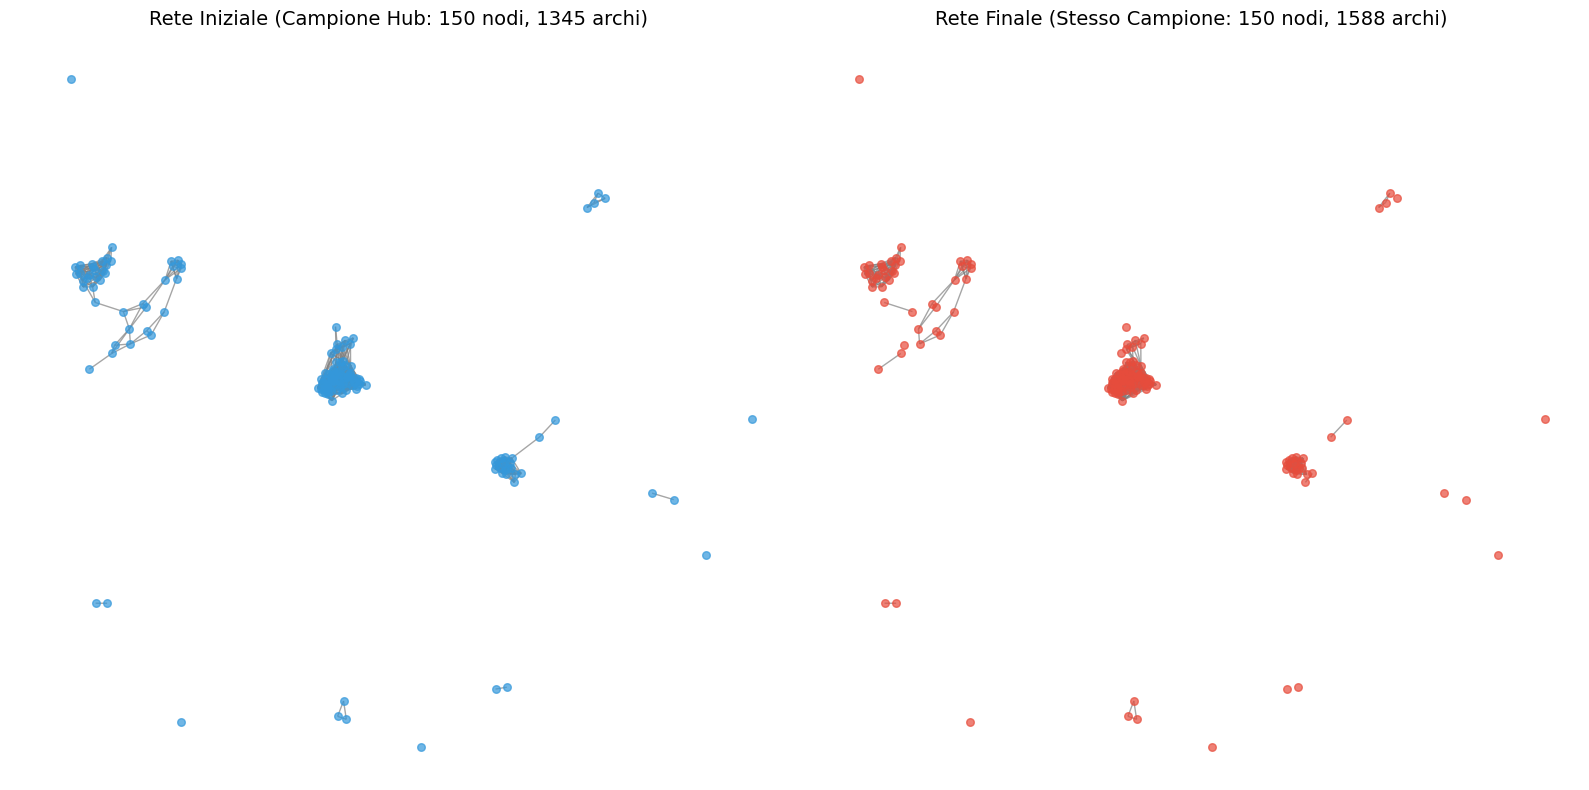
\includegraphics[width=\textwidth]{rete_iniziale_finale.png}
    \caption{Confronto tra la topologia della rete allo step iniziale (sinistra, 150 nodi campionati sugli hub, 1\,345 archi) e allo step 129 (destra, stesso campione, 1\,588 archi), al termine della co-evoluzione. L'immagine si riferisce alla run di controllo; la topologia della run con intervento è praticamente identica, come confermano ECI e modularità.}
    \label{fig:rete-iniziale-finale}
\end{figure}

Il confronto visivo conferma quanto osservato nelle metriche aggregate delle Fasi 2 e 3. Nella rete iniziale (sinistra) il campione si presenta come un insieme di piccoli cluster densi e ben separati tra loro, con pochissimi legami di lungo raggio: la struttura a compartimenti stagni tipica di una rete di co-autoraggio accademico organizzata per sotto-discipline. Nella rete finale (destra), a parità di nodi, emergono alcuni elementi distintivi:

\begin{itemize}[leftmargin=*]
    \item \textbf{Concentrazione degli archi sugli hub:} la rete nel suo complesso mantiene la stessa densità (26\,246 archi), ma il campione di hub guadagna archi (da 1\,345 a 1\,588, $+18\%$). Il rewiring sostituisce archi senza aggiungerne: quelli nuovi tendono a collegare nodi centrali, mentre quelli rimossi stanno altrove nella rete.
    \item \textbf{Cluster più compatti:} i nuovi archi si concentrano all'interno dei cluster già esistenti, che risultano più densi, invece di creare ponti tra gruppi diversi. È l'effetto del rewiring guidato dalla GNN: nuovi archi nascono tra agenti che hanno sviluppato posizioni simili nello spazio degli embedding, ed è coerente con la crescita di modularità ed Echo Chamber Index.
    \item \textbf{Stabilità della periferia:} i nodi periferici a basso grado (coppie isolate o singoli nodi) restano sostanzialmente invariati. Sui 150 hub osservati, il rewiring non stravolge la disposizione dei gruppi, ma ne aumenta la coesione interna.
\end{itemize}

Questo pattern visivo è coerente con il quadro emerso dalle metriche numeriche: il rewiring della GNN non stravolge la topologia della rete, ma la ``rifinisce'' selettivamente, sostituendo circa il 10\% degli archi in 100 step e rendendo più coesi sia le community originarie sia, in misura maggiore, i gruppi di opinione. L'intervento di fact-checking, nella finestra osservata, agisce invece sul livello cognitivo (stati e opinioni) e non sulla struttura fisica del grafo.

\subsection{Conclusioni Generali}
La pipeline implementata in \texttt{progettoASM} rappresenta un solido paradigma di simulazione sociale in cui l'intelligenza artificiale generativa smette di essere un semplice strumento di supporto e diviene il motore stesso dell'evoluzione di rete.

L'architettura, attraverso la successione ordinata delle fasi, mostra come la co-evoluzione tra topologia e cognizione agentica non sia soltanto una curiosità teorica, ma un fenomeno misurabile e tracciabile quantitativamente. La coerenza strutturale del campionamento (verificata nella Fase 0), la scalabilità garantita dall'uso ottimizzato di \texttt{vLLM} (impiegato con continuità nelle Fasi 1, 2 e 3) e il disegno sperimentale con run di controllo conferiscono al framework una notevole robustezza metodologica.

I risultati principali si possono riassumere in quattro punti:
\begin{enumerate}
    \item Gli agenti LLM producono una dinamica di diffusione realistica: crescita rapida, saturazione intorno al 41\% dei nodi e comparsa spontanea di resistenti, che arrivano quasi a pareggiare gli infetti.
    \item La co-evoluzione rafforza le echo chamber, soprattutto quelle di \textbf{opinione}: la belief assortativity sale da 0.27 a 0.66, mentre l'Echo Chamber Index strutturale cresce in misura molto minore (da 0.83 a 0.87). L'indice strutturale da solo sottostimerebbe la segregazione: è necessario affiancare metriche basate sulle opinioni.
    \item Un intervento tardivo con 20 fact-checker (0.4\% dei nodi) protegge circa 160 suscettibili (il 16\% di quelli rimasti), in linea con la stima della selezione, ma lascia invariata la popolazione infetta già consolidata. Con le regole del modello, il fact-checking funziona come prevenzione più che come cura.
    \item L'intervento non riduce la polarizzazione: la rafforza leggermente, perché sposta nodi neutrali su posizioni nette.
\end{enumerate}

\paragraph{Limitazioni.} Ogni configurazione è stata eseguita una sola volta: con un costo di circa 6 minuti per step non è stato possibile ripetere le run con seed diversi, e gli effetti più piccoli richiederebbero repliche per essere confermati. Il seed per richiesta rende ripetibili le risposte a parità di prompt, ma vLLM non garantisce il determinismo completo con batching variabile. L'obiettivo di selezione dei seed considera l'effetto immediato dei fact-checker sui vicini, non la dinamica futura (ricadute, rewiring, risposte dell'LLM). Infine, il rewiring a densità costante ha staccato dalla rete 85 piccoli gruppi di nodi in 100 step (153 allo step 129): un vincolo di connettività sulle rimozioni renderebbe la rete più realistica.

I risultati ottenuti, archiviati in \texttt{metrics\_history.csv}, \texttt{metrics\_history\_control.csv} e nei report della Fase 3, costituiscono la base per ulteriori indagini scientifiche. In futuro, il sistema potrà essere esteso integrando algoritmi di \textit{GNN Explainer} per interpretare visivamente quali legami stiano effettivamente guidando la polarizzazione, testando diverse architetture di agenti LLM per osservare se differenti ``personalità'' algoritmiche conducano a velocità di convergenza verso l'omofilia sensibilmente diverse, o esplorando budget di fact-checker più ampi e finestre di attivazione più precoci, prima che il contagio si stabilizzi, per verificare a quali condizioni l'intervento riesca a ridurre anche la popolazione infetta.

\subsection{Riepilogo Esecutivo della Pipeline}
Al termine di ciascuna run, la pipeline stampa un riepilogo consuntivo che raccoglie in forma compatta i principali indicatori dell'esperimento, dalla costruzione del sottografo fino all'intervento finale. Di seguito i valori delle due run della Fase 3:

\begin{tcolorbox}[colback=gray!5, colframe=gray!60, title=\texttt{PIPELINE COMPLETATA}, fonttitle=\bfseries, sharp corners]
\begin{tabular}{lll}
                     & \textbf{Con fact-checker} & \textbf{Controllo} \\
    Nodi simulati    & 5\,000 & 5\,000 \\
    Archi            & 26\,246 & 26\,246 \\
    Community        & 415 (Q baseline $= 0.8265$) & 415 (Q baseline $= 0.8265$) \\
    Step Fase 2      & 100 & 100 \\
    Infection rate   & $0.4064 \rightarrow 0.4040$ & $0.4064 \rightarrow 0.4048$ \\
    ECI              & $0.8741 \rightarrow 0.8855$ & $0.8741 \rightarrow 0.8858$ \\
    Seed fact-checker & 20 nodi & 0 nodi \\
    Copertura efficace & 0.0010 & 0.0000 \\
\end{tabular}
\end{tcolorbox}

Il riepilogo conferma, in forma aggregata, il quadro delineato nelle sezioni precedenti: la rete parte da una condizione di forte segregazione comunitaria (415 community, $Q=0.8265$); nei 30 step finali l'infection rate scende di pochi millesimi in entrambe le run, mentre l'ECI cresce in modo quasi identico nelle due run, a riprova che l'intervento incide sulla dimensione cognitiva e non su quella strutturale della rete.
\end{document}
